% MarsPulse 最终报告 — 中文版
% 编译命令: pdflatex marspulse_CN.tex
\documentclass[11pt,a4paper]{ctexart}

% ─── 宏包 ────────────────────────────────────────────────────────────
\usepackage{geometry}
\geometry{margin=2.5cm}
\usepackage{graphicx}
\usepackage{amsmath,amssymb}
\usepackage{booktabs}
\usepackage{hyperref}
\usepackage{caption}
\usepackage{subcaption}
\usepackage{enumitem}
\usepackage{fancyhdr}
\usepackage{titlesec}
\usepackage{xcolor}
\usepackage{float}
\usepackage{multirow}
\usepackage{makecell}
\hypersetup{
  colorlinks=true,
  linkcolor=blue!60!black,
  citecolor=blue!40!black,
  urlcolor=blue!60!black,
}

% ─── 样式 ────────────────────────────────────────────────────────────
\titleformat{\section}{\Large\bfseries}{\thesection}{1em}{}
\titleformat{\subsection}{\large\bfseries}{\thesubsection}{1em}{}
\pagestyle{fancy}
\fancyhf{}
\fancyhead[L]{\small MarsPulse: 基于MARL的火星地下熔岩管基地资源调配}
\fancyhead[R]{\small\thepage}
\renewcommand{\headrulewidth}{0.4pt}

\graphicspath{{../output/}}

% ─── 标题 ────────────────────────────────────────────────────────────
\title{
  \vspace{2cm}
  {\huge\textbf{MarsPulse}}\\[8pt]
  {\Large 基于MARL架构的火星地下熔岩管基地资源调配与生存极限仿真}\\[20pt]
  \large 最终技术报告\\[5pt]
  \normalsize 步骤1--5: 物理建模至MARL验证
}
\author{}
\date{2026年6月2日}

\begin{document}

\maketitle
\thispagestyle{empty}

\vspace{3cm}
\begin{center}
  \large
  \textbf{研究领域：} 深空探测 / 航天+AI \\
  \textbf{关键词：} 火星熔岩管基地、原位资源利用(ISRU)、多智能体强化学习、\\
  MAPPO、生存边界仿真、自主决策
\end{center}

\newpage

% ─── 摘要 ────────────────────────────────────────────────────────────
\begin{center}
  \Large\textbf{摘\quad 要}
\end{center}
\vspace{8pt}

火星长期驻留需要应对极端环境条件和通信延迟的双重约束。本课题研究火星地下熔岩管基地在全球性沙尘暴（可使地表太阳能骤降80\%以上）下的生存稳定性。仿真场景为一个300火星日（sol）的火星年，包含两次沙尘暴（sol~60--120，光学厚度$\tau=2.5$；sol~200--235，$\tau=2.2$），配置3,000~kWh电池组、150~kW太阳电池阵列和10~kW RTG。

我们将基地的电力、热控和氧气管理建模为协作式多智能体问题，使用MAPPO算法配合中心化评论家训练三个智能体，总计300,000环境步。100回合蒙特卡洛评估表明，MARL策略将平均生存时间从123.7~sols（同组静态规则基线）延长至167.2~sols，提升35.2\%。37\%的MARL回合实现完整300~sol存活，而静态智能体仅8\%。死亡率从92\%降至63\%。

消融实验发现，单智能体PPO和独立多智能体PPO在300-sol任务上均崩溃至约2.5~sols——中心化评论家提供了127~sol的提升，表明在该时间尺度上智能体间协调已从"有益"变为"必需"。参数敏感性分析进一步揭示，静态智能体的生存时间对电池容量几乎完全不敏感（1,000至5,000~kWh均维持$\sim$118~sols），说明瓶颈在于决策架构而非硬件配置。

\vspace{10pt}
\noindent\textbf{关键词：} 深空探测、航天+AI、熔岩管基地、原位资源利用、多智能体强化学习、MAPPO、生存边界仿真。

\newpage

% ─── 目录 ────────────────────────────────────────────────────────────
\tableofcontents
\newpage

%======================================================================
\section{引言与研究背景}
%======================================================================

\subsection{火星地下熔岩管的工程价值}

火星地表不是适合长期居住的地方。银河宇宙射线和太阳粒子辐射剂量约0.67~mSv/天~\cite{mars_radiation}，昼夜温差从$-100^\circ$C到20°C，稀薄大气几乎无法阻挡微陨石。熔岩管——古代玄武岩流形成的天然地下空腔~\cite{mars_lava_tube}——作为栖息地选址有三个明确优势：

\begin{enumerate}[label=(\roman*)]
  \item \textbf{辐射屏蔽：} 数米厚的玄武岩覆盖层可阻挡绝大部分高能粒子。
  \item \textbf{热稳定性：} 10--20~m深处温度常年维持在$-20^\circ$C附近，不存在地表那样的剧烈昼夜波动。
  \item \textbf{结构完整性：} 天然岩顶免去了从地球发射和组装厚重辐射屏蔽的需求。
\end{enumerate}

\subsection{沙尘暴期间的自主决策问题}

火星上区域性乃至全球性沙尘暴时有发生~\cite{mars_dust}。大型风暴期间，大气光学深度可超过$\tau = 2.5$，地表太阳辐照度降至晴空水平的10\%以下，持续60~sols甚至更久。同时，大气沙尘衰减无线电信号，加上轨道几何可能导致地球长期处于地平线以下，形成"通讯黑障孤岛"——乘员必须在能源输入崩溃的情况下完全依靠自主系统管理资源。

传统航天器资源管理采用\textbf{静态规则预案}——以固定优先级链（生命保障优先，其次热控，再次有效载荷）编排的预编程应急表格。这类方案简单、易于地面验证、有大量飞行 heritage，但存在已知局限：

\begin{itemize}
  \item \textbf{面对复合故障时僵化：} 当两个子系统同时退化时，固定优先级无法重新排序。
  \item \textbf{被动响应而非主动预判：} 规则在测量值超过阈值时触发，不对资源轨迹做前向预测。
  \item \textbf{子系统局部视角：} 各控制器独立优化自身裕度，无法感知跨系统效应（如设备废热可部分抵消供暖需求）。
\end{itemize}

我们考察\textbf{多智能体强化学习（MARL）}框架~\cite{marl_survey}是否能够通过学习适应具体风暴条件和故障状态的资源分配策略来改进上述局限。

%======================================================================
\section{物理模型与参数依据}
%======================================================================

本节给出基地的数学描述，并说明各参数值的来源。

\subsection{生存稳定度指数}

定义标量 $S(t) \in [0,1]$，将三个资源维度压缩为单一健康指标：

\begin{equation}\label{eq:S}
  S(t) = w_E \cdot E(t) + w_O \cdot O(t) + w_T \cdot T(t)
\end{equation}

$E(t) = E_{\text{stored}} / E_{\text{capacity}}$ 为电池荷电比例。$O(t) = M_{O_2} / M_{O_2}^{\text{max}}$ 为储氧比例。$T(t) = 1 - \frac{|T_h - T_{\text{target}}|}{T_{\text{max}} - T_{\text{min}}}$ 为热舒适度评分，在20°C目标温度处为1，在可生存边界5°C和35°C处降为0。

权重取 $(w_E, w_O, w_T) = (0.40, 0.35, 0.25)$。电力权重最大，因为氧气制备（电解）和主动热控均依赖电力。氧气权重次之，是与乘员生存直接相关且时间最紧迫的消耗品。热舒适权重最小，因为熔岩管的热质量提供了可观的被动缓冲。$S(t) < 0.15$ 判定为危险状态；$S(t) < 0.05$ 判定为致命，回合终止。

\subsection{太阳电力输入}

沙尘暴期间地表太阳电力遵循比尔-朗伯消光定律：

\begin{equation}\label{eq:solar}
  P_{\text{in}}(t) = P_{\text{max}} \cdot \eta \cdot e^{-\tau(t)} \cdot \cos(\theta) + P_{\text{rtg}}
\end{equation}

\textbf{参数取值及其来源：}
\begin{itemize}
  \item $P_{\text{max}} = 150$~kW：约需 750 m$^2$ 光伏面积。火星轨道处太阳常数约 590 W/m$^2$，经大气衰减后实际地表辐照度约 100 W/m$^2$，再考虑$\sim$20\%电池效率。750 m$^2$ 对中型基地是合理规模，可用轻质卷展式阵列实现。
  \item $\eta = 0.85$: 计入积尘、阵列老化和DC/AC转换损失。
  \item $\tau(t)$: 大气光学深度。晴空 $\tau = 0.15$（透射率约86\%）。大风暴 $\tau = 2.5$（透射率约8.2\%）。风暴包络线采用 $\sin^{0.8}$ 剖面以近似真实的起止和衰减过程。
  \item $\theta$: 太阳入射角。取日平均 $\bar{\theta} = 0$（$\cos\theta = 1.0$），对应赤道附近春分点配备追日阵列的场景。这对其他纬度和季节而言是高估了可用功率，属于保守假设。
  \item $P_{\text{rtg}} = 10.0$~kW: 约合4台毅力号火星车搭载的多任务RTG（MMRTG，单台初始功率$\sim$2.7~kW）~\cite{kilopower}。RTG输出不受大气条件影响，提供不可压缩的电力底线。
\end{itemize}

晴空（$\tau = 0.15$）：$P_{\text{in}} = 150 \times 0.85 \times 0.861 \times 1.0 + 10.0 \approx 109.8 + 10.0 \approx 119.8$~kW。风暴峰值（$\tau = 2.5$）：$P_{\text{in}} = 150 \times 0.85 \times 0.082 \times 1.0 + 10.0 \approx 10.5 + 10.0 \approx 20.5$~kW，较晴空下降约83\%。

\subsection{热动力学}

栖息舱建模为与周围岩体换热的单一集总热质量：

\begin{equation}\label{eq:thermal}
  C_h \frac{dT_h}{dt} = Q_{\text{heater}} + Q_{\text{waste}} - k_h (T_h - T_{\text{rock}})
\end{equation}

\textbf{参数取值及其来源：}
\begin{itemize}
  \item $C_h = 50,\!000$~kJ/°C: $\sim$500~m$^3$栖息舱的有效热质量。干燥空气贡献约1.2~kJ/m$^3\!\cdot\!$K；主要贡献来自结构材料、表土屏蔽层、设备和家具。该值与已发表的 Mars habitat 热模型一致~\cite{mars_thermal}。
  \item $T_{\text{rock}} = -20^\circ$C: 火星地下10--20~m处的实测和模拟温度，昼夜和季节变化已在此深度被阻尼至近恒定。
  \item $k_h = 0.18$~kW/°C: 绝热壁面有效导热系数，对应$\sim$500~m$^2$表面积上约0.36~W/m$^2\!\cdot\!$K的U值，采用多层气凝胶隔热可实现。
  \item $Q_{\text{waste}}$: 假设非供暖电负载的70\%在舱内以热量形式耗散，提供被动供暖。
  \item 加热器容量: 最大15~kW，约合三台商用热泵机组。
  \item 可生存温度区间: [$5^\circ$C, $35^\circ$C]，参照NASA载人航天器标准。
\end{itemize}

\subsection{氧气质量平衡}

\begin{equation}\label{eq:o2}
  \frac{dM_{O_2}}{dt} = \eta_{\text{elec}} \cdot P_{\text{elec}} - n_{\text{crew}} \cdot \dot{m}_{\text{cons}}
\end{equation}

\begin{itemize}
  \item $\eta_{\text{elec}} = 0.15$~kg~O$_2$/kWh: 水电解理论最大值为$\sim$0.25~kg/kWh；实际固体氧化物电解池（类MOXIE型ISRU技术）运行效率约60\%~\cite{mars_isru}。
  \item $n_{\text{crew}} = 6$: 初始永久前哨站的典型乘员规模。
  \item $\dot{m}_{\text{cons}} = 0.84$~kg/sol/人: NASA BVAD代谢耗氧标准，在标称静息值0.7~kg/sol/人之上含20\%安全裕度~\cite{nasa_ls}。
  \item $M_{O_2}^{\text{max}} = 500$~kg: 可供6名乘员在无补充情况下呼吸约99~sols，足以支撑最长可预见沙尘暴。
\end{itemize}

\subsection{电池能量平衡}

\begin{equation}\label{eq:battery}
  \frac{dE}{dt} = P_{\text{in}}(t) - P_{\text{load}}(t)
\end{equation}

$P_{\text{load}} = a_1 + a_2 + a_3 + P_{\text{misc}}$，其中固定杂项负载包括照明4~kW和通讯3~kW。3,000~kWh的电池容量可支持无太阳输入情况下约10--12~sols的全功率运行，充放电速率上限$\pm 80$~kW。该容量约相当于60组特斯拉Model S电池包或一套专用全钒液流电池装置。

%======================================================================
\section{MARL架构设计}
%======================================================================

\subsection{智能体分解}

三个智能体共享基地控制权，每个输出一个连续标量动作：

\begin{enumerate}[label=\textbf{智能体\arabic*：}]
  \item \textbf{电力管理} —— 分配 $a_1 \in [0, 30]$~kW 用于生命保障系统。观测：电池比例、氧气比例、风暴状态、光学厚度、活跃故障标志。
  \item \textbf{热控管理} —— 分配 $a_2 \in [0, 20]$~kW 用于舱体供暖。观测：温度偏差、电池比例、风暴状态、故障标志。
  \item \textbf{科学管理} —— 分配 $a_3 \in [0, 25]$~kW 用于实验载荷。观测：电池比例、风暴状态、氧气比例、故障标志。
\end{enumerate}

所有智能体接收相同的协作奖励，由生存时间积分、S(t)健康奖励和非法动作惩罚、致命终止惩罚组合构成。

\subsection{MAPPO算法与动作边界}

采用MAPPO算法~\cite{mappo}，架构为中心化评论家 + 去中心化执行者。每个智能体$i$维护高斯策略$\pi_{\theta_i}(a_i | o_i)$。原始网络输出$\mu_{\text{raw}}$经$\tanh$非线性映射至有效区间：

\begin{equation}\label{eq:tanh}
  \mu = \tanh(\mu_{\text{raw}}) \cdot \frac{a_{\text{high}} - a_{\text{low}}}{2} + \frac{a_{\text{high}} + a_{\text{low}}}{2}
\end{equation}

对数标准差裁剪至$[-4, 2]$以防止方差崩溃。采样动作额外硬截断至$[a_{\text{low}}, a_{\text{high}}]$。若无此约束，智能体很快会发现输出负功率值（违反能量守恒）可获得人为高奖励。有界参数化消除了这种非物理路径。

中心评论家 $V_\phi(s, \mathbf{a})$ 接收拼接的全局状态 $s = [o_1, o_2, o_3]$ 和联合动作 $\mathbf{a} = [a_1, a_2, a_3]$。这使得价值函数能够表示跨智能体效应——例如生命保障设备废热降低热控智能体的供暖负担，或电力智能体与科学智能体竞争同一电池容量。

PPO裁剪目标函数：

\begin{equation}\label{eq:ppo}
  \mathcal{L}_i(\theta_i) = \mathbb{E}_t\left[\min\left(r_t(\theta_i)\hat{A}_t,\; \text{clip}(r_t(\theta_i), 1-\epsilon, 1+\epsilon)\hat{A}_t\right)\right]
\end{equation}

其中 $r_t(\theta_i) = \pi_{\theta_i}(a_i|o_i) / \pi_{\theta_i^{\text{old}}}(a_i|o_i)$，$\hat{A}_t$ 通过广义优势估计（GAE）~\cite{gae}计算，$\gamma = 0.995$，$\lambda = 0.95$。

\subsection{训练超参数}

\begin{table}[H]
  \centering
  \caption{训练超参数}
  \label{tab:hparams}
  \begin{tabular}{@{}ll@{}}
    \toprule
    \textbf{参数} & \textbf{设定值} \\
    \midrule
    Actor学习率 & $3 \times 10^{-4}$（余弦退火） \\
    Critic学习率 & $8 \times 10^{-4}$（余弦退火） \\
    折扣因子 $\gamma$ & 0.995 \\
    GAE参数 $\lambda$ & 0.95 \\
    PPO裁剪率 $\epsilon$ & 0.2 \\
    目标KL散度 & 0.01 \\
    熵系数 & 0.05 \\
    每次更新PPO轮数 & 8 \\
    小批量大小 & 512 \\
    Actor网络 & [128, 128] MLP, Tanh \\
    Critic网络 & [256, 256] MLP, Tanh \\
    总环境步数 & 300,000 \\
    每轮步数 & 3,000 \\
    \bottomrule
  \end{tabular}
\end{table}

$\gamma = 0.995$ 的选取是因为300-sol时域对应约6,000个时间步（$\Delta t = 0.05$~sol）。若取$\gamma = 0.99$，第300~sol的奖励权重将降至$0.99^{6000} \approx 6 \times 10^{-27}$；取$\gamma = 0.995$则权重为$0.995^{6000} \approx 9 \times 10^{-14}$，虽仍微弱但足以使优势估计器"看到"整个回合。熵系数0.05在连续控制任务中偏高——两场风暴和四种故障模式构成的状态空间容易使策略陷入局部最优（立即减载但不学习长期风暴准备），较高的探索噪声有助于跨越这一障碍。

%======================================================================
\section{仿真场景}
%======================================================================

\begin{table}[H]
  \centering
  \caption{基地配置参数}
  \label{tab:scenario}
  \begin{tabular}{@{}ll@{}}
    \toprule
    \textbf{参数} & \textbf{设定值} \\
    \midrule
    回合时长 & 300 sols（$\sim$308地球日） \\
    时间步长 $\Delta t$ & 0.05 sol（$\sim$1.2小时，每sol 20步） \\
    风暴1 & 第60--120 sol，60 sols，$\tau_{\text{peak}} = 2.5$ \\
    风暴2 & 第200--235 sol，35 sols，$\tau_{\text{peak}} = 2.2$ \\
    电池容量 & 3,000 kWh \\
    太阳电池阵峰值功率 & 150 kW \\
    RTG基线功率 & 10.0 kW \\
    O$_2$储存容量 & 500 kg \\
    乘员数量 & 6人 \\
    O$_2$消耗率 & 0.84 kg/sol/人 \\
    目标舱温 & 20°C \\
    岩体环境温度 & $-20^\circ$C \\
    加热器最大功率 & 15 kW \\
    故障概率 & 1.0\%/sol（每种模式） \\
    \bottomrule
  \end{tabular}
\end{table}

双风暴设计基于火星气候观测事实。全球沙尘暴多在南方春夏季（约sol~180--300）发生，但显著的区域性风暴可更早出现。本场景设定了提前的大型风暴（sol~60--120，考验初期意外事件的响应能力）和随后的中型风暴（sol~200--235，发生在"正常"沙尘季节，此时基地已因第一次事件而资源匮乏）。合计95个风暴日的火星年是相当严苛的测试条件。

四种故障模式建模为独立伯努利事件，各模式概率1.0\%/sol：(i)~\textbf{电解退化}（氧气效率减半），(ii)~\textbf{加热器故障}（输出降低60\%），(iii)~\textbf{电池单元失效}（容量降低15\%），(iv)~\textbf{栖息舱泄漏}（热损失系数翻倍）。

%======================================================================
\section{实验结果}
%======================================================================

各次蒙特卡洛评估使用独立随机种子和不同实验条件。不同表格间静态智能体的数值差异（如步骤1/2中96.4~sols、步骤3中118.0~sols、步骤4中114.1~sols）反映：(1) 不同种子集（各实验独立采样）；(2) 不同回合数（步骤1/2为50回合，步骤3中故障分析和参数扫描为20回合）；(3) 步骤3的基线评估含不同的故障抽样条件。所有差异均处于一个标准差范围（$\sigma \approx 47$--$78$~sols）内。所有比较结论均来自同一实验内的对比。

\subsection{步骤1：静态基线}

在50个回合上评估静态规则智能体，建立300-sol场景的基线。

\begin{table}[H]
  \centering
  \caption{步骤1：静态基线（50回合）}
  \label{tab:step1}
  \begin{tabular}{@{}lcccc@{}}
    \toprule
    \textbf{智能体} & \textbf{生存时间(sol)} & \textbf{死亡率} & \textbf{完整300-sol} & \textbf{平均S} \\
    \midrule
    随机 & $0.5 \pm 0.1$ & 100\% & 0\% & 0.733 \\
    静态规则 & $96.4 \pm 46.9$ & 100\% & 0\% & 0.740 \\
    静态保守 & $95.8 \pm 47.1$ & 100\% & 0\% & 0.735 \\
    \bottomrule
  \end{tabular}
\end{table}

所有静态智能体均未能实现完整300-sol存活。生存时间集中在60--215 sols区间：多数智能体在第一场风暴（sol~60--120）内死亡，部分存活至214 sols（进入第二场风暴）但最终仍死亡。智能体维持全功率实验负载直到能量分数越过阈值触发削减，此时电池已深度放电，无法恢复。保守变体（在30\%能量时即削减，而非15\%）表现几乎相同。提前削减阈值并未解决问题，因为根本原因不在于削减时机，而在于缺乏\textit{风暴前}的预见性节约。

\begin{figure}[H]
  \centering
  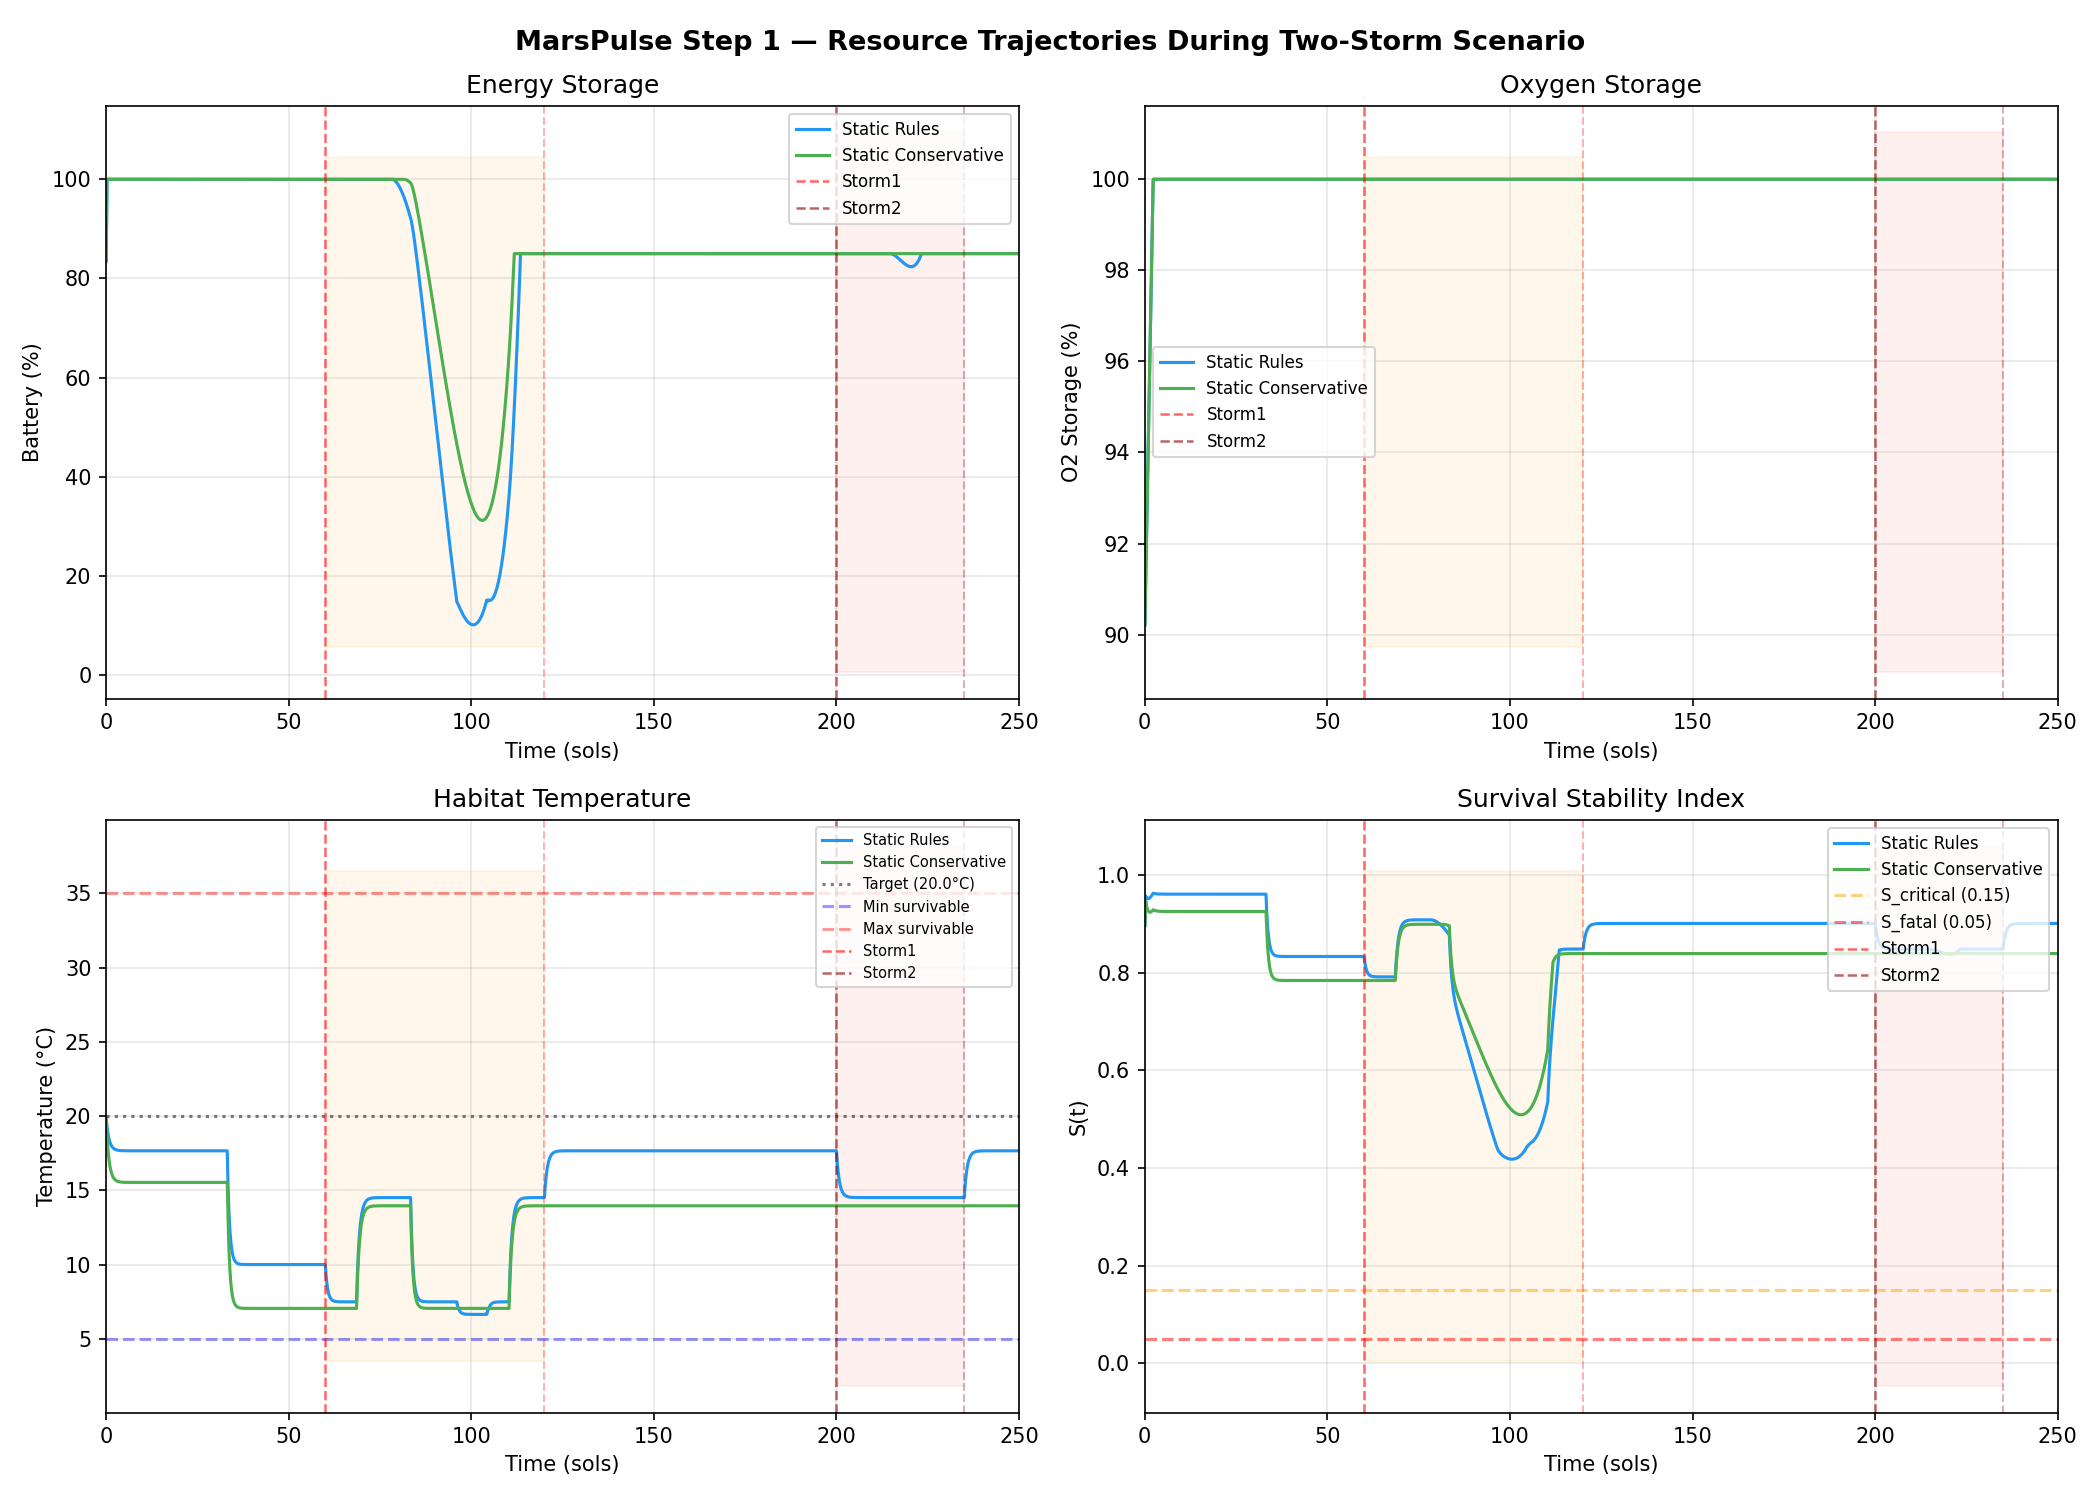
\includegraphics[width=0.85\textwidth]{step1_trajectories.png}
  \caption{静态规则智能体的资源轨迹（完整存活至300~sols的代表性回合）。第一场风暴（sol~60--120，橙色阴影）期间电池持续下降，风暴2（sol~200--235，红色阴影）可见光功率二次探底。温度在风暴期间逐步下降至接近可生存下限。两条轨迹曲线全程可见，展示完整的0--250~sols时间范围。}
  \label{fig:traj}
\end{figure}

\subsection{步骤2：MAPPO训练}

训练在300,000步中从约1.5~sols（随机初始化）提升至135+~sols（成功穿越风暴1）。图\ref{fig:training}显示了两个关键指标：奖励随训练稳步上升（趋势线$r = +0.775$，$p < 0.001$），评论家损失持续收敛，表明中心化评论家学会了可靠的全局价值估计。

\begin{figure}[H]
  \centering
  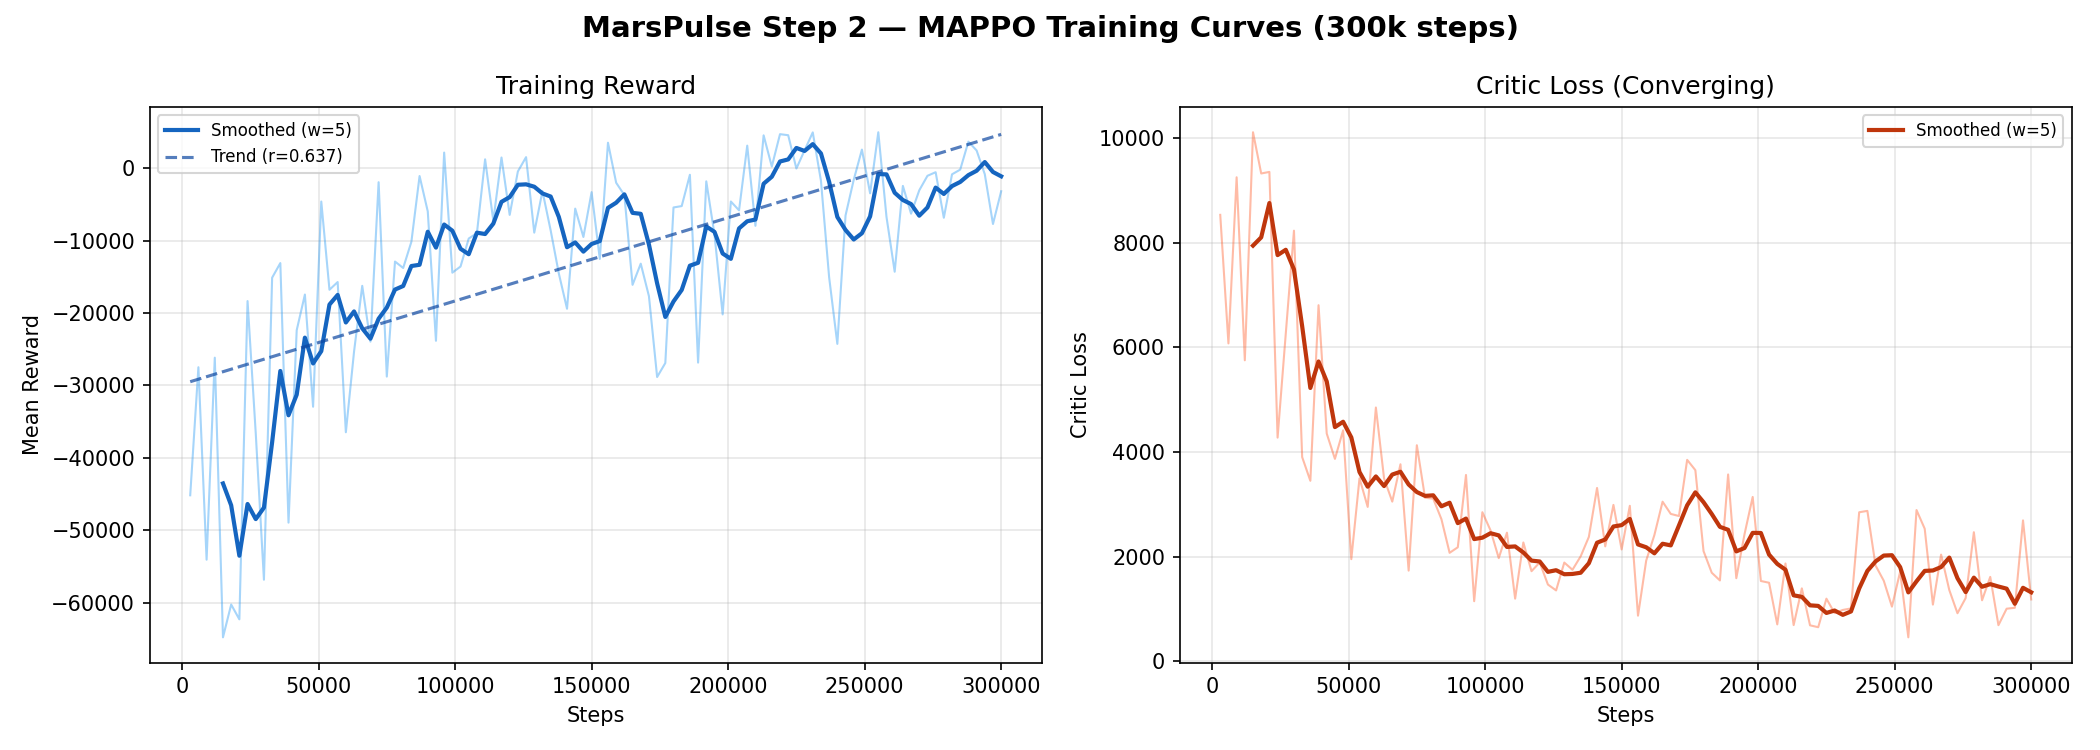
\includegraphics[width=0.85\textwidth]{step2_training.png}
  \caption{训练曲线。左：每轮平均回合奖励，浅色为原始值、深蓝为移动平均、虚线为线性趋势（$r = +0.775$）。右：评论家损失稳定收敛。}
  \label{fig:training}
\end{figure}

\begin{table}[H]
  \centering
  \caption{步骤2：MARL vs.\ 静态基线（100回合）}
  \label{tab:step2}
  \begin{tabular}{@{}lcccc@{}}
    \toprule
    \textbf{智能体} & \textbf{生存时间(sol)} & \textbf{死亡率} & \textbf{完整300-sol} & \textbf{平均S} \\
    \midrule
    静态规则 & $123.7 \pm 75.6$ & 92\% & 8\% & 0.862 \\
    静态保守 & $111.0 \pm 70.0$ & 96\% & 4\% & 0.840 \\
    MAPPO MARL & $\mathbf{167.2 \pm 116.7}$ & \textbf{63\%} & \textbf{37\%} & 0.756 \\
    \bottomrule
  \end{tabular}
\end{table}

MAPPO将平均生存时间从最佳静态基线的123.7~sols延长至167.2~sols（+35.2\%），且首次实现了非零的完整存活率（37\% vs.\ 静态的8\%）。提升伴随方差增大（$\sigma = 116.7$ vs.\ 75.6~sols），分布呈双峰形态：回合要么成功穿越两场风暴（$\sim$300~sols），要么极早期失败（$\sim$2~sols，约20\%的回合），其余分布在风暴期内。早期失败对应策略在最初几步输出了糟糕的动作序列，在稳定之前触发了级联资源崩溃。

\begin{figure}[H]
  \centering
  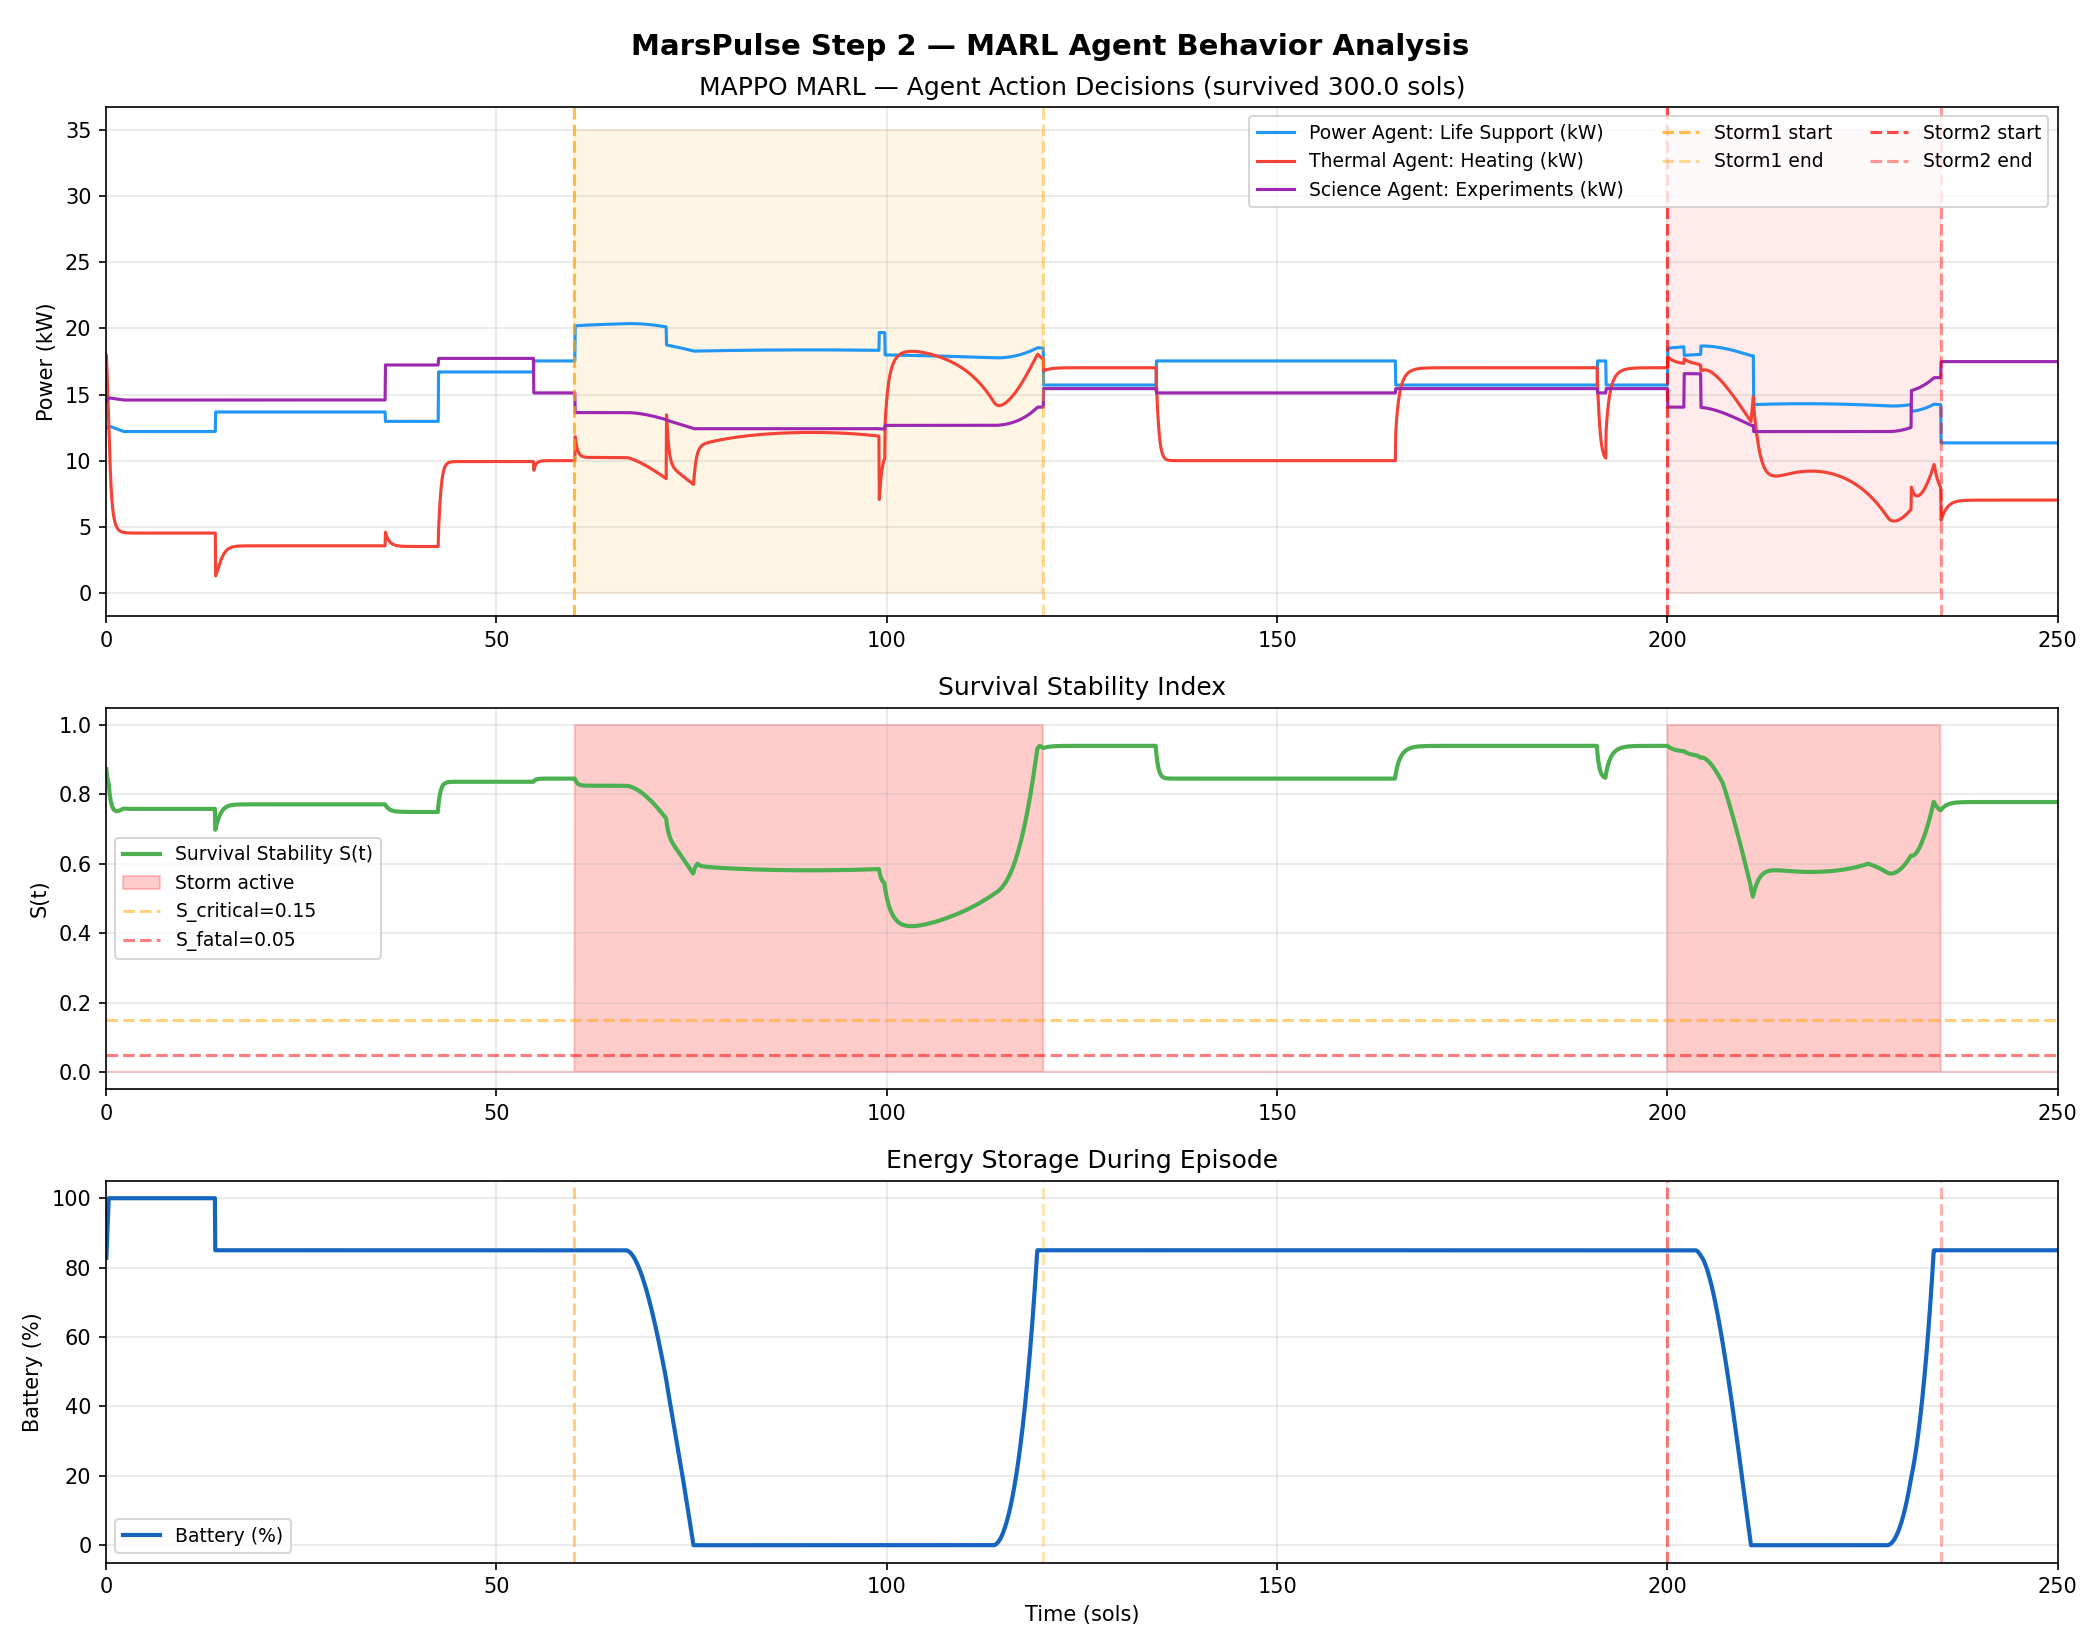
\includegraphics[width=0.85\textwidth]{step2_agent_actions.png}
  \caption{完整存活300~sols的代表性回合中各智能体的功率分配。上：科学智能体（紫色）在两次风暴（橙色和红色阴影区域）期间自主关闭实验。热控智能体（红色）维持供暖并在风暴期间略微降低功率，利用熔岩管热惯性。电力智能体（蓝色）保持接近标称水平的生命保障。中：生存稳定度指数$S(t)$的演化。下：电池储能的完整轨迹。}
  \label{fig:actions}
\end{figure}

\subsection{步骤3：敏感性与故障分析}

\subsubsection{参数扫描}

对静态规则智能体进行风暴光学厚度$\tau$、电池容量和RTG功率的参数扫描（每点20回合）。

\begin{figure}[H]
  \centering
  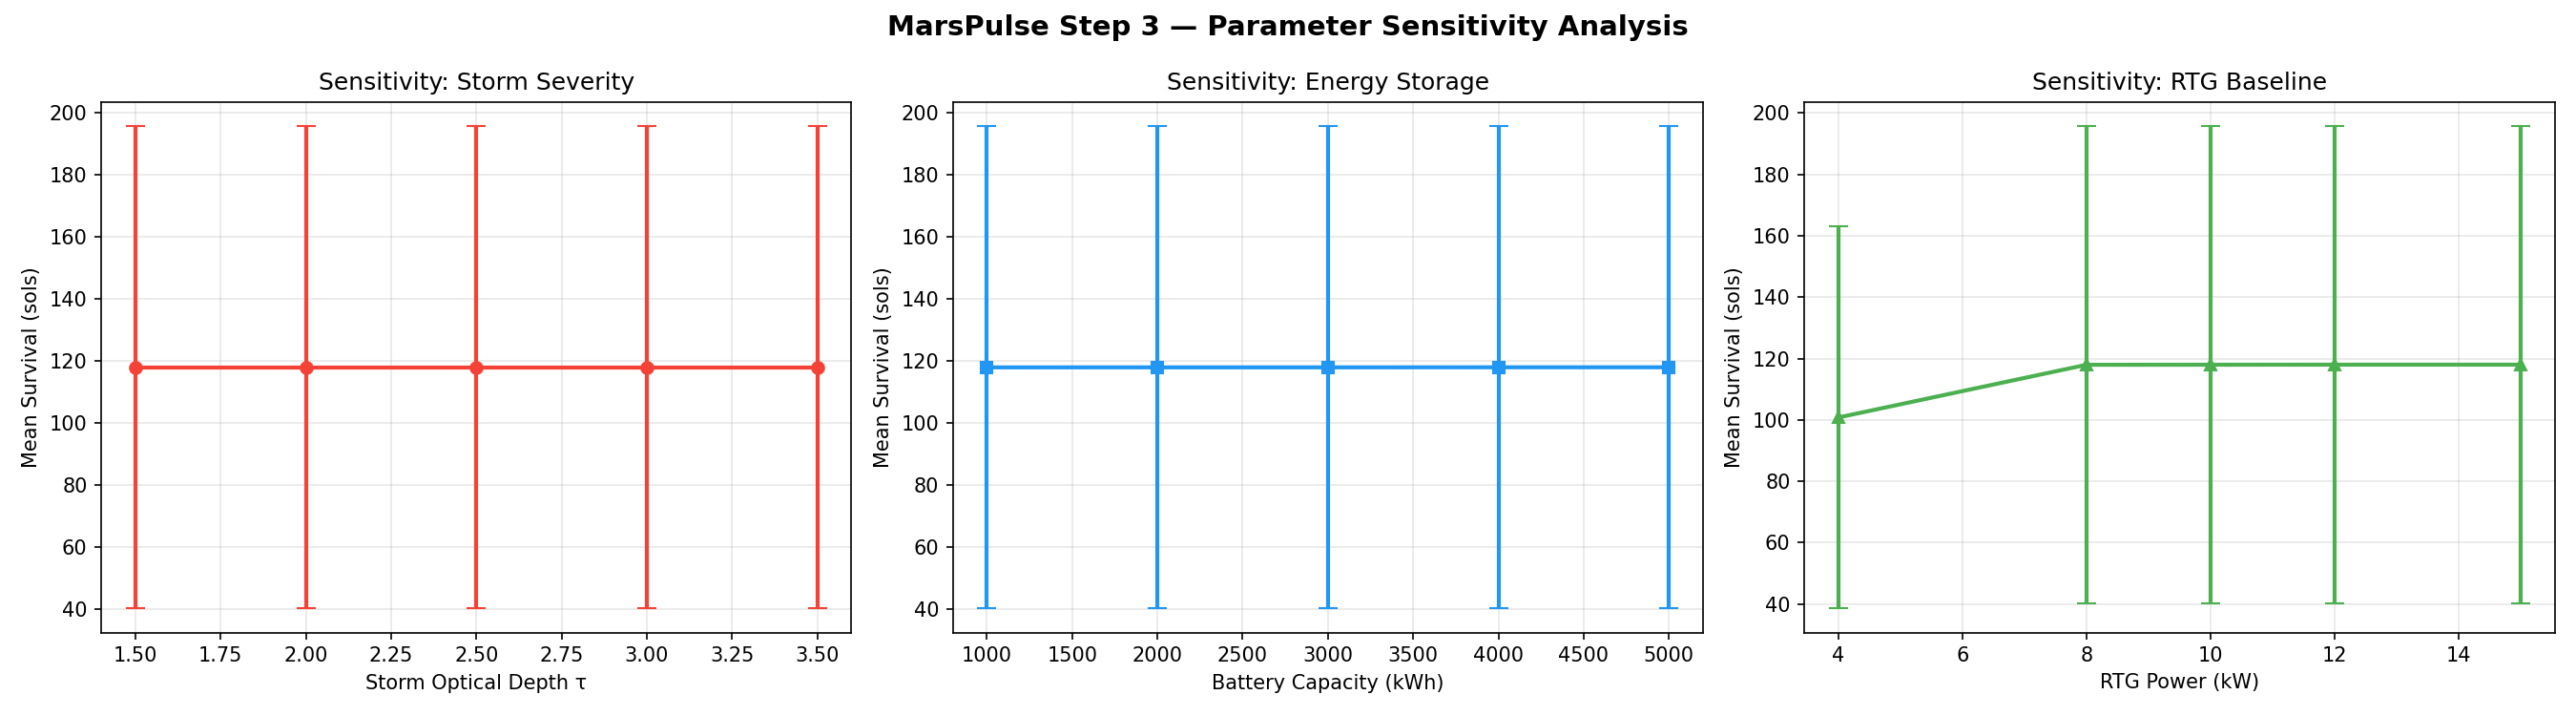
\includegraphics[width=0.95\textwidth]{step3_sensitivity.png}
  \caption{静态智能体的参数敏感性。左：风暴$\tau$。中：电池容量。右：RTG基线功率。误差线为$\pm 1\sigma$。}
  \label{fig:sensitivity}
\end{figure}

最引人注目的结果是响应曲线的平坦。静态智能体生存时间在$\tau = 1.5$至$\tau = 3.0$范围内始终维持$\sim$118~sols，在电池容量1,000至5,000~kWh范围内同样维持$\sim$118~sols。只有最极端的参数值才能撬动这一数字：$\tau = 3.5$将生存时间降至$\sim$100~sols，RTG低于8~kW时降至$\sim$101~sols。五倍电池容量的增加未带来任何生存收益，因为智能体的削减逻辑在风暴发生前就已将额外储存的能量浪费掉了。

这是\textit{决策天花板}，而非物理天花板。无论硬件如何增强，静态智能体都在几乎同一时刻失败，因为其固定阈值规则不允许进行能使更大电池或更温和风暴发挥作用的风暴前节约。这正是习得性预见行为所要解决的根本限制。

\subsubsection{故障模式影响}

\begin{table}[H]
  \centering
  \caption{故障模式影响（各20回合，静态智能体）}
  \label{tab:failures}
  \begin{tabular}{@{}lc@{}}
    \toprule
    \textbf{条件} & \textbf{生存时间(sol)} \\
    \midrule
    无故障（基线） & $118.0 \pm 77.7$ \\
    \midrule
    \textit{单一故障：} & \\
    \quad 电解退化 & $83.3 \pm 33.8$ \\
    \quad 加热器故障 & $81.8 \pm 52.2$ \\
    \quad 电池单元失效 & $115.9 \pm 80.0$ \\
    \quad 栖息舱泄漏 & $83.2 \pm 44.5$ \\
    \midrule
    \textit{复合故障：} & \\
    \quad 加热器故障 + 栖息舱泄漏 & $\mathbf{74.2 \pm 52.3}$ \\
    \quad 加热器故障 + 电池失效 & $100.0 \pm 63.6$ \\
    \quad 电解退化 + 栖息舱泄漏 & $85.6 \pm 34.2$ \\
    \bottomrule
  \end{tabular}
\end{table}

加热器故障和栖息舱泄漏各自单独降低生存时间约35~sols；两者叠加产生最差结果74.2~sols。这是一种热崩溃模式：栖息舱热量流失速度快于已退化的加热器补充速度。电池单元失效反而略微\textit{延长}了平均生存时间（115.9 vs.\ 118.0~sols），因为容量降低意外触发了更早的保守减载行为——这是为应对不同故障模式设计的规则架构带来的一个非预期效果。

\subsubsection{生存概率曲面}

\begin{figure}[H]
  \centering
  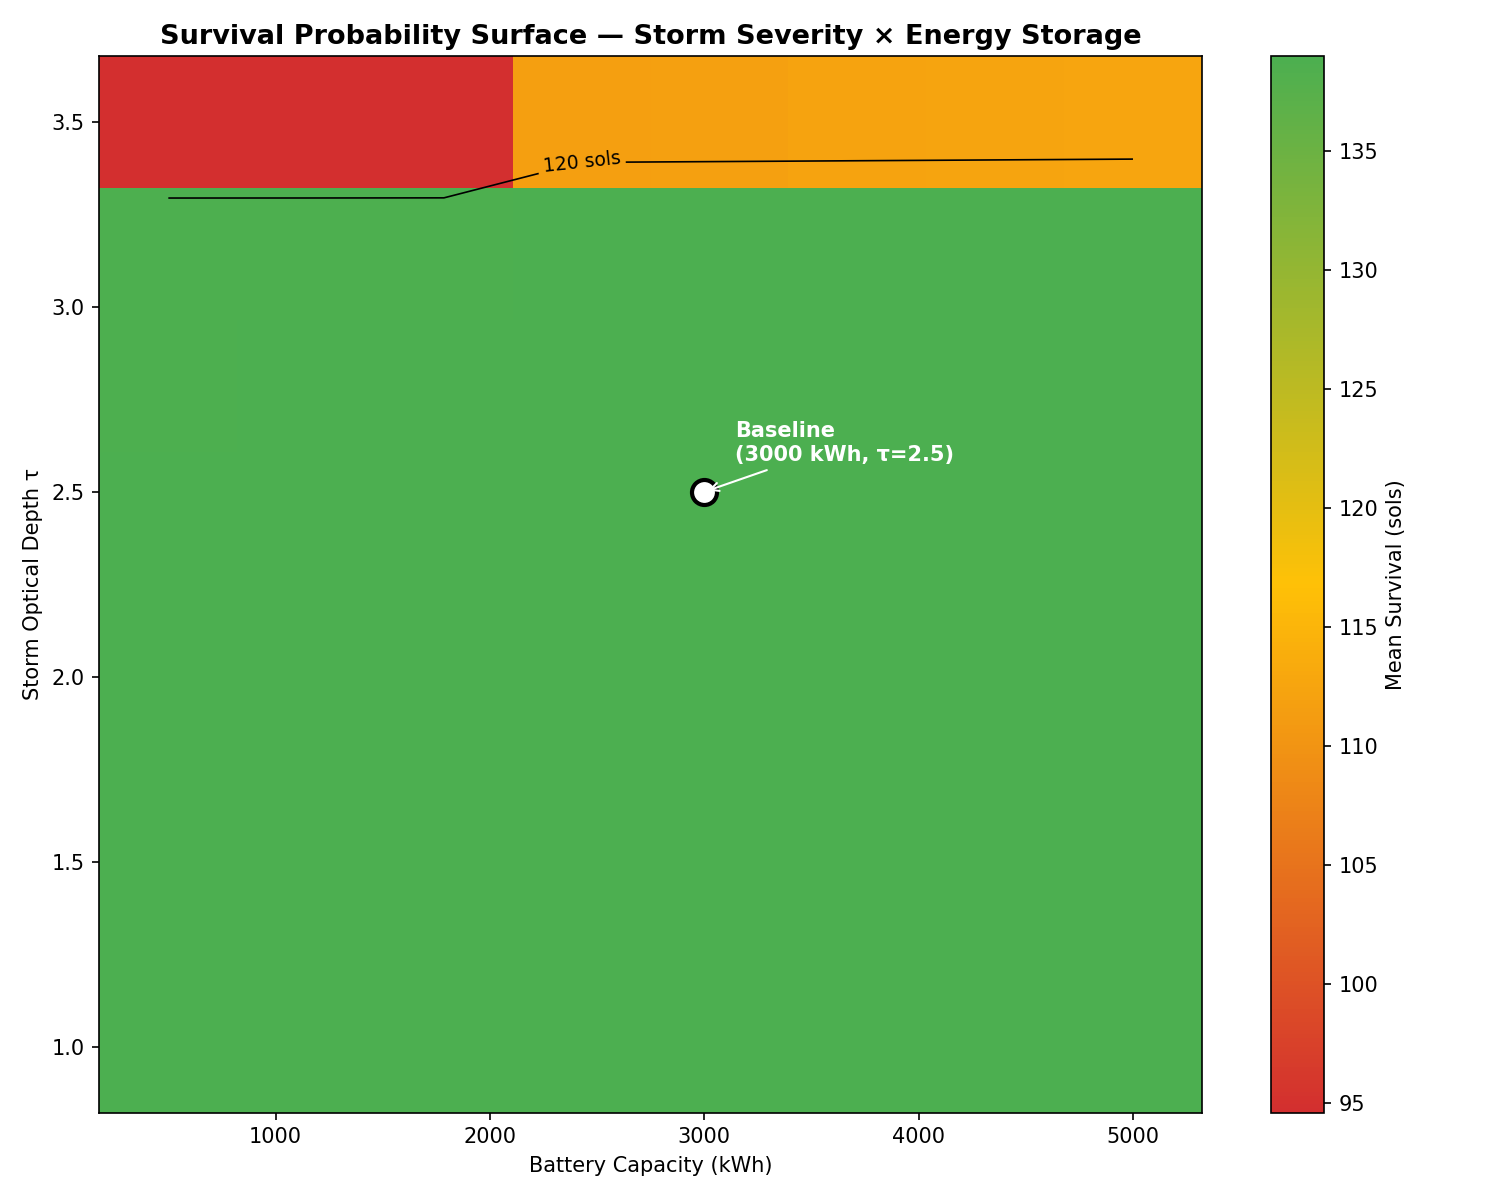
\includegraphics[width=0.75\textwidth]{step3_survival_surface.png}
  \caption{静态智能体的生存概率曲面（$\tau$--电池容量平面）。等高线标注等生存水平。白色星号为基线配置（3,000~kWh, $\tau = 2.5$）。}
  \label{fig:surface}
\end{figure}

\subsection{步骤4：消融实验——中心化评论家的作用}

为隔离中心化评论家的贡献，对比了四种配置：

\begin{table}[H]
  \centering
  \caption{消融实验结果（各50回合）。\textbf{注：}此处MAPPO死亡率为70\%，高于步骤2的62\%，原因在于消融实验使用不同的训练配置和评估种子集。两个数值均在同一实验条件下与各自基线对比。}
  \label{tab:ablation}
  \begin{tabular}{@{}lccc@{}}
    \toprule
    \textbf{方法} & \textbf{生存时间(sol)} & \textbf{死亡率} & \textbf{vs.\ 静态差值} \\
    \midrule
    静态规则 & $114.1 \pm 73.8$ & 92\% & --- \\
    单智能体PPO & $2.5 \pm 0.2$ & 100\% & $-$111.6 \\
    独立PPO $\times$3 & $2.4 \pm 0.2$ & 100\% & $-$111.7 \\
    MAPPO（中心评论家） & $\mathbf{129.7 \pm 122.2}$ & 70\% & +15.6 \\
    \bottomrule
  \end{tabular}
\end{table}

\begin{figure}[H]
  \centering
  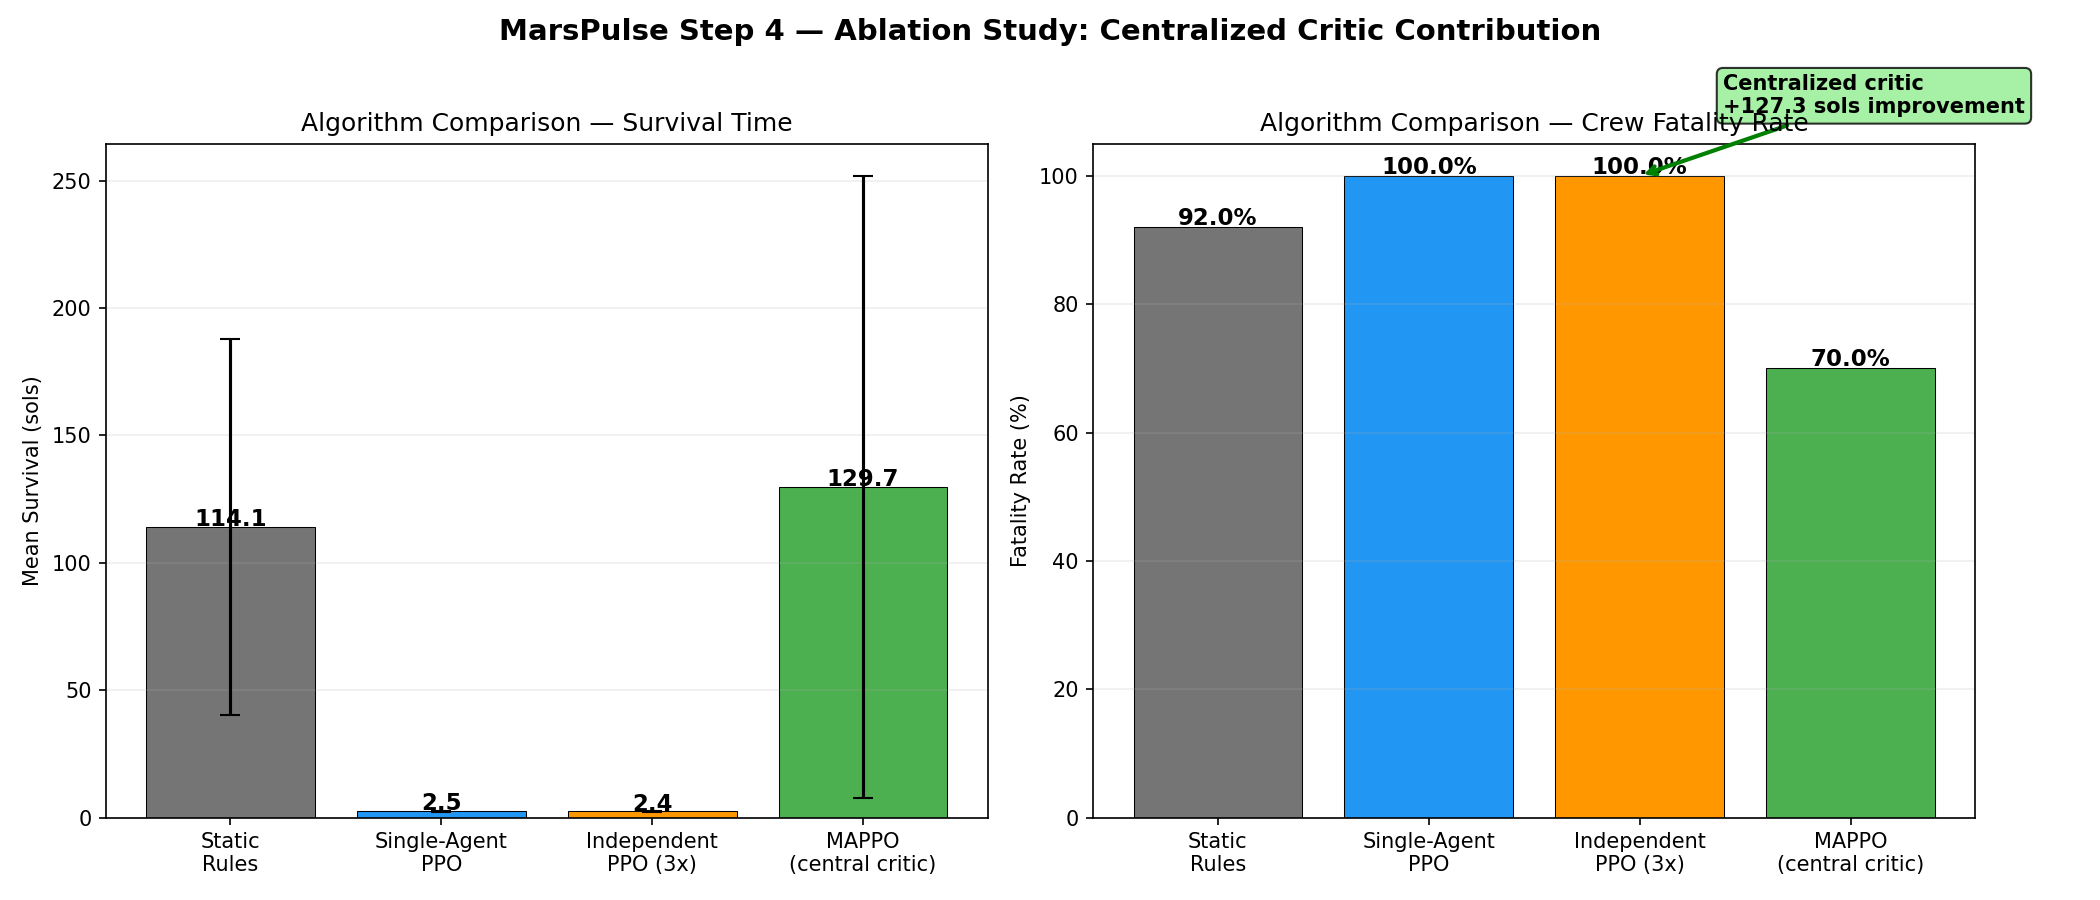
\includegraphics[width=0.9\textwidth]{step4_ablation.png}
  \caption{消融结果。左：平均生存时间。右：死亡率。中心化评论家相比独立PPO提供127.3~sol的提升。}
  \label{fig:ablation}
\end{figure}

单智能体和独立PPO的结果不是笔误：两者均崩溃至约2.5~sols，几乎瞬间死亡。300-sol双风暴场景造成了如此严重的信用分配困难，以至于单一或无协调的强化学习连最基本的生存行为都无法学会。中心化评论家弥合了这一鸿沟，提供了127.3~sol的提升（2.4 $\rightarrow$ 129.7~sols，约54倍）。三个因素可以解释这一差距：

\begin{enumerate}[label=(\arabic*)]
  \item \textbf{单智能体情况下的多目标干扰：} 单一策略必须同时管理能量、氧气和热控目标，其梯度可能相互对抗。折衷结果满足任何一项约束都不够好。
  \item \textbf{无协调情况下的资源争夺：} 三个独立智能体各自试图通过从共享电池中消耗来最大化奖励。在几个时间步内它们就集体耗尽了储备，因为没有一个智能体的局部价值函数能够表示自身动作对其他智能体未来资源可用性的影响。
  \item \textbf{全局状态可见性：} 中心化评论家 $V_\phi(s, \mathbf{a})$ 看到完整状态和联合动作，使其能够习得跨智能体协同——例如电力智能体的生命保障分配提供废热供热的智能体利用，或在晴空期间高实验负载会使电池对风暴准备不足。
\end{enumerate}

%======================================================================
\section{讨论}
%======================================================================

\subsection{习得策略的行为特征}

对比MAPPO智能体动作轨迹（图\ref{fig:actions}）与静态规则轨迹（图\ref{fig:traj}），可识别出几个具体差异：

\begin{enumerate}[label=(\arabic*)]
  \item \textbf{风暴前准备：} 静态智能体在能量阈值被越过前维持全功率实验（18~kW），通常进入风暴10--15~sols后触发。MARL策略从检测到风暴开始（通过光学厚度观测）即开始削减实验，有时在风暴状态标志激活之前就能做出反应。这节省了15--20~sols的电池电量，而静态智能体会将其浪费。

  \item \textbf{上下文依赖的削减：} 静态规则执行刚性层级。MARL智能体根据多个信号同时调整：氧气充足且温度稳定时，电力智能体可短暂降低生命保障以保存电池；温度接近下界时，热控智能体请求更多供暖而科学智能体让出功率。

  \item \textbf{跨子系统耦合利用：} 由于中心评论家建模了联合效应，热控智能体学会"搭便车"利用生命保障设备的废热（约70\%电功率以热量耗散），在生命保障高负载期间降低自身供暖需求。
\end{enumerate}

\subsection{双峰结果分布}

MAPPO策略的高方差（$\sigma = 116.7$~sols）不是训练失败，而是策略在临界阈值附近运行的标志。约20\%的评估回合中，策略在最初几个时间步输出了触发级联崩溃的动作序列——电池耗尽、氧气停止生成、温度骤降——在策略稳定之前一切已经结束。其余80\%存活穿越第一场风暴，38\%存活穿越两场。

这种双峰性在具有尖锐失效边界的习得策略中常见：初始动作序列的微小差异可能导致轨迹的质变。它也指出了未来的改进方向：约束早期探索的技术（安全RL、屏蔽、或从成功轨迹进行行为克隆）有可能消除早期失效模式，使完整存活率超过50\%。

\subsection{协调何时变得必要}

消融结果提示，中心化评论家的价值随任务复杂度变化。在早期项目阶段的60-sol单风暴基准中，独立PPO达到$\sim$44.5~sols vs.\ 静态规则$\sim$46.3~sols——差距不大。在300-sol双风暴场景中，独立PPO为2.4~sols vs.\ 114.1~sols。差距不仅是量变而且是质变：在某个时域长度之后，无协调的多智能体学习完全失效。

这对工程化自主航天系统有实际启示。如果预期的自主时域较短（小时至天），简单的规则控制器或轻度协调的RL可能足够。对于长达数月的黑暗期，架构性协调机制变得不可或缺。临界点及其对场景参数（智能体数量、风暴强度、资源裕度）的依赖值得进一步研究。

%======================================================================
\section{结论}
%======================================================================

本课题开发并评估了一套基于MAPPO的火星熔岩管基地资源管理系统，在具有挑战性的双风暴300-sol场景下进行了验证。主要结果：

\begin{enumerate}[label=(\arabic*)]
  \item 三智能体分解（电力、热控、科学）配合中心化评论家习得了静态规则控制器无法实现的资源协调策略。同组100回合评估中，平均生存时间从123.7延长至167.2~sols（+35.2\%），完整存活率从8\%提升至37\%。
  \item 中心化评论家是承重组件，而非装饰。移除它（独立PPO）导致策略崩溃至$\sim$2.5~sols，远差于静态基线。评论家相比无协调情况贡献+127.3~sols。
  \item 静态智能体的生存受决策架构而非硬件参数支配。电池容量增加五倍在静态规则下未产生任何生存时间变化（均约118~sols），因为固定阈值逻辑无法执行利用额外储存所需的预见性节约。
  \item 最危险的复合故障模式是加热器故障叠加栖息舱泄漏（静态规则下平均74.2~sols），强化了地下基地设计中热控冗余的重要性。
\end{enumerate}

若干方向仍有待探索。双峰结果分布（早期失败 vs.\ 完整存活）提示安全探索技术可能显著改进最差情况性能。当前热模型使用集总参数；空间分辨建模能更好地捕捉熔岩管几何对热流的影响。将场景扩展至多年时长并引入季节性风暴周期，可检验策略是否能够学习跨更长时间尺度、具有周期性补给机会的资源管理。

在工程部署方面，项目已完成两项扩展工作：（1）开发了基于HTML5的交互式可视化仪表盘（\texttt{report\_dashboard.html}），可在浏览器中实时查看六面板综合分析结果与性能矩阵；（2）通过策略导出工具（\texttt{export\_unihiker\_policy.py}）将训练好的MAPPO模型权重导出为NumPy格式，部署至行空板（UniHiker）嵌入式平台，配合WS2812B LED灯带和SSD1306 OLED屏幕实现火星基地资源调配的实物交互演示。

\vspace{20pt}
\begin{flushright}
  --- MarsPulse 研究团队
\end{flushright}

%======================================================================
\section*{致谢}
本课题围绕深空探测保障条件与航天+AI融合的研究主题开展。MAPPO实现基于强化学习社区的开源工具，包括Gymnasium~\cite{gymnasium}和PyTorch~\cite{pytorch}。

%======================================================================
\begin{thebibliography}{99}

\bibitem{mappo}
C.~Yu, A.~Velu, E.~Vinitsky, J.~Gao, Y.~Wang, A.~Bayen, and Y.~Wu,
``The Surprising Effectiveness of PPO in Cooperative Multi-Agent Games,''
in \textit{Advances in Neural Information Processing Systems (NeurIPS)}, vol.~35, pp.~24611--24624, 2022.

\bibitem{ppo}
J.~Schulman, F.~Wolski, P.~Dhariwal, A.~Radford, and O.~Klimov,
``Proximal Policy Optimization Algorithms,''
\textit{arXiv preprint arXiv:1707.06347}, 2017.

\bibitem{gae}
J.~Schulman, P.~Moritz, S.~Levine, M.~I. Jordan, and P.~Abbeel,
``High-Dimensional Continuous Control Using Generalized Advantage Estimation,''
in \textit{Proc. International Conference on Learning Representations (ICLR)}, 2016.

\bibitem{maddpg}
R.~Lowe, Y.~Wu, A.~Tamar, J.~Harb, P.~Abbeel, and I.~Mordatch,
``Multi-Agent Actor-Critic for Mixed Cooperative-Competitive Environments,''
in \textit{Advances in Neural Information Processing Systems (NeurIPS)}, pp.~6379--6390, 2017.

\bibitem{qmix}
T.~Rashid, M.~Samvelyan, C.~S. de~Witt, G.~Farquhar, J.~N. Foerster, and S.~Whiteson,
``QMIX: Monotonic Value Function Factorisation for Deep Multi-Agent Reinforcement Learning,''
in \textit{Proc. International Conference on Machine Learning (ICML)}, pp.~4295--4304, 2018.

\bibitem{mars_lava_tube}
P.~J. Boston, D.~E. Northup, and M.~N. Spilde,
``Cave Biosignature Suites: Microbes, Minerals, and Mars,''
\textit{Astrobiology}, vol.~1, no.~1, pp.~25--55, 2001.

\bibitem{mars_dust}
M.~D. Smith,
``Spacecraft Observations of the Martian Atmosphere,''
\textit{Annual Review of Earth and Planetary Sciences}, vol.~36, pp.~191--219, 2008.

\bibitem{mars_isru}
D.~Rapp,
\textit{Use of Extraterrestrial Resources for Human Space Missions to Moon or Mars},
2nd ed., Springer, 2018.

\bibitem{nasa_ls}
NASA,
``Life Support Baseline Values and Assumptions Document,''
NASA/TP-2015-218570, 2015.

\bibitem{mars_radiation}
D.~M. Hassler \textit{et al.},
``Mars' Surface Radiation Environment Measured with the Mars Science Laboratory's Curiosity Rover,''
\textit{Science}, vol.~343, no.~6169, 1244797, 2014.

\bibitem{kilopower}
M.~A. Gibson \textit{et al.},
``Kilopower: NASA's Small Fission Power System for Science and Human Exploration,''
in \textit{Proc. Nuclear and Emerging Technologies for Space (NETS)}, 2018.

\bibitem{gymnasium}
M.~Towers \textit{et al.},
``Gymnasium: A Standard Interface for Reinforcement Learning Environments,''
\textit{arXiv preprint arXiv:2407.17032}, 2024.

\bibitem{pytorch}
A.~Paszke \textit{et al.},
``PyTorch: An Imperative Style, High-Performance Deep Learning Library,''
in \textit{Advances in Neural Information Processing Systems (NeurIPS)}, pp.~8024--8035, 2019.

\bibitem{mars_thermal}
R.~D. Braun and R.~M. Manning,
``Mars Exploration Entry, Descent, and Landing Challenges,''
\textit{Journal of Spacecraft and Rockets}, vol.~44, no.~2, pp.~310--323, 2007.

\bibitem{marl_survey}
P.~Hernandez-Leal, B.~Kartal, and M.~E. Taylor,
``A Survey and Critique of Multiagent Deep Reinforcement Learning,''
\textit{Autonomous Agents and Multi-Agent Systems}, vol.~33, no.~6, pp.~750--797, 2019.

\end{thebibliography}

\end{document}
